\documentclass[11pt]{article}

\usepackage{graphicx}
\usepackage[numbers]{natbib}

\title{Assignment 1 report - INF-1400}
\author{Edvard Pedersen}



\begin{document}

\maketitle

\section{Introduction}

\emph{Give a short summary of the assignment.}

In this assignment, we make a breakout clone using OOP principles, with an emphasis on using classes and methods. 

\section{Technical Background}

\emph{Mention the technologies used, this is only a sentance or two, unless you're using a different language/library/whatever}

For this assignment, Python 3.4\cite{python} was used, which is an interpreted programming language, which supports the OOP principles. In addition, an SDL wrapper...

\section{Design}

\emph{Give an overarching view of the structure of your solution.}

Describe how your objects fit together, a figure like figure 1 must be included, and you should refer to it in the design section. Remember to refer to figures, such as Figure 1 below, in your text.

\begin{figure}[h]
	\centering
	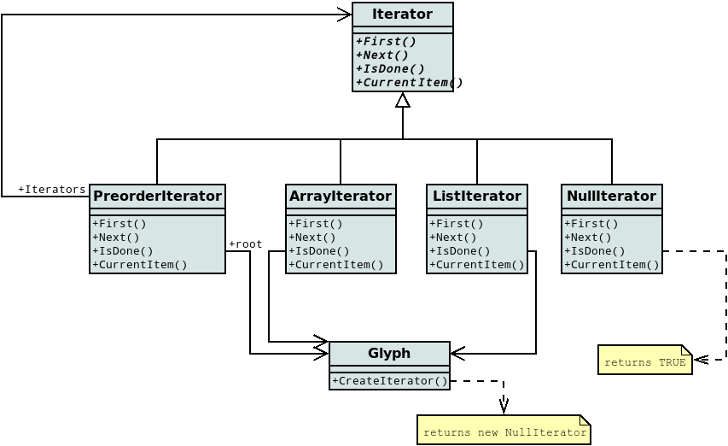
\includegraphics[width=\textwidth]{UML.png}
	\caption{Example UML diagram, taken from \cite{umlsource}}
	\label{umlfig}
\end{figure}

\section{Implementation}

\emph{Describe implementation details, particularly those that are not obvious choices}

For the implementation of the paddle, the visual representation on the screen is different from the internal representation used for collision detection, by representing the paddle in this way we achieve... 


\section{Evaluation}

\emph{Examine if your submission fulfils the requirements and what shortcomings exist.}

In this solution, all requirements are fulfilled, but collision detection between the ball and paddle is inaccurate, due to differences between the visual representation and the implementation...

\section{Discussion}

\emph{Discuss what could be done better, problems you had, experiences etc. (we also appreciate feedback on the assignment or group sessions) }

The implementation of the paddle-ball collision could be done \emph{some other way}, but due to \emph{some reason}, the current implemetation is better.

After spending two days trying to write the report in \LaTeX, I gave up, and wrote it in Word instead.

\section{Conclusion}

\emph{Sum up the previous sections.}

I have implemented a solution that fulfills the requirements, the implementation is moderately buggy, but does not crash too much.


\bibliographystyle{plainnat}
\bibliography{example.bib}

\end{document}
